\graphicspath{{../../S17_Inegalite_triangulaire/Images/}}

\themeG
\chapter{L'inégalité triangulaire}
\label{S17}

\programme%
   {\item Triangle : inégalité triangulaire.}
   {\item Mettre en \oe uvre ou écrire un protocole de construction d’une figure géométrique.}

\vfill

\begin{debat}{Débat :  des instruments de navigation astronomique anciens}
   De tous temps, les hommes ont cherché à se repérer. Avant l’avènement de l'électronique et des GPS, de multiples instruments ont pu exister, par exemple : 
   \tcblower
      \begin{tabular}{*{4}{C{3.6}}}
         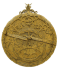
\includegraphics[height=3cm]{astrolabe} & 
\includegraphics[height=3cm]{boussole}  & 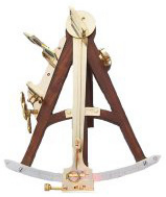
\includegraphics[height=3cm]{octant} & 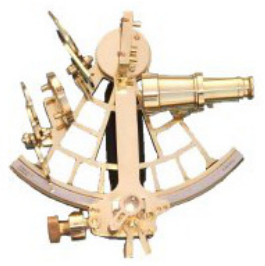
\includegraphics[height=3cm]{sextant} \\
         Astrolabe : & Boussole : & Octant : & Sextant : \\
         représentation plane de la sphère céleste & indique le nord magnétique & mesure la hauteur des corps célestes (45°) & mesure la hauteur des corps célestes (60°) \\
         Antiquité & {\small XIII}\up{e} & {\small XVIII}\up{e} & {\small XVIII}\up{e} \\
   \end{tabular}
\end{debat}

\hfill {\gray Vidéo : \href{https://www.youtube.com/watch?v=E0KvuFx0Mr8}{\bf Du kamal au GPS 1} et \href{https://www.youtube.com/watch?v=Jv21tvyZokk}{\bf Du kamal au GPS 2}, chaîne Youtube du {\it Musée national de la marine}.}


%%% Approche %%%
\begin{Maquette}[Cours]{Theme={Activité d'approche},Couleur={SteelBlue}}

   \AAtitre{Avec des allumettes}

      {\it Objectifs : construire des triangles sous contraintes.}

      \begin{AActivite}

         Devant vous, vous avez dix allumettes. Pour chacune des questions suivantes, faire la construction si elle est possible avec des allumettes puis faire un dessin pour schématiser la situation.
         \begin{enumerate}
            \item
            \begin{enumerate}
               \item Aligner quatre allumettes en les plaçant les unes à côté des autres.
               \medskip
               \begin{center}
                  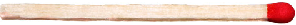
\includegraphics[width=3cm]{allumette}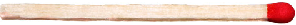
\includegraphics[width=3cm]{allumette}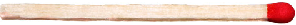
\includegraphics[width=3cm]{allumette}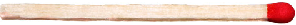
\includegraphics[width=3cm]{allumette}
               \end{center}
               \medskip
               \item À partir de ce segment de longueur 4 allumettes, construire un triangle dont les deux autres côtés ont pour longueur trois allumettes. \par \vskip2.5cm
               \item En utilisant les dix allumettes, construire un triangle différent du précédent dont un des côtés a pour longueur quatre allumettes. Quelles sont les longueurs de ses côtés ? \par \vskip2.5cm
            \end{enumerate}
            \item En utilisant les dix allumettes, est-il possible de construire un triangle dont un des côtés a pour longueur six allumettes ? sept allumettes ? Expliquer. \par \vskip2.5cm
            \item En utilisant les dix allumettes, peut-on construire un triangle dont un côté a pour longueur cinq allumettes ? Que constate-t-on dans ce cas ? \par \vskip2.5cm
            \item On veut maintenant construire un triangle de périmètre 12 allumettes dont les côtés ont pour longueur un nombre entier d'allumettes. Donner toutes les solutions possibles ainsi que la nature des triangles. \vspace*{2.5cm} 
         \end{enumerate}

   \end{AActivite}

\end{Maquette}


%%% cours %%%
\begin{Maquette}[Cours]{Theme={Trace écrite},Couleur={0.4[SteelBlue,Black]}}

   %%%1
   \section{L'inégalité triangulaire}

      \begin{propriete*}{}
         Dans un triangle, la longueur d'un côté est toujours inférieure à la somme des longueurs des deux autres côtés. S'il y a égalité, alors les trois points sont alignés et le triangle est \og plat \fg.
      \end{propriete*}

      \begin{exemple*}{}
         \begin{minipage}{6cm}
            {\small
            \begin{pspicture}(-0.75,-0.3)(3.5,2.5)
               \pstGeonode[CurveType=polygon,PointSymbol=none,PosAngle={180,90,0}](0,0){A}(2.5,2){C}(3.5,0){B}
               \pstLabelAB[offset=-3mm]{A}{B}{\Lg{3,5}}
               \pstLabelAB{A}{C}{\Lg{3,2}}
               \pstLabelAB{C}{B}{\Lg{2,2}}
            \end{pspicture}}
         \end{minipage}
         \begin{minipage}{10cm}
            Dans le triangle $ABC$, on a :
            \begin{itemize}
               \item $AC =\Lg{3,2}$ et $AB+BC =\Lg{5,7}$ donc $AC\leq AB+BC$ ;
               \item $CB =\Lg{2,2}$ et $CA+AB =\Lg{6,7}$ donc $CB\leq CA+AB$ ;
               \item $BA =\Lg{3,5}$ et $BC+CA =\Lg{5,4}$ donc $BA\leq BC+CA$.
            \end{itemize}
         \end{minipage}
      \end{exemple*}
   
      Remarque : dans la pratique, on vérifie seulement que la longueur du plus grand côté est plus grande que la somme des longueurs des deux autres côtés.
   
   
   %%%2
   \section{Construction de triangles}
   
      Pour construire un triangle, il faut au minimum trois données :
      \begin{itemize}
         \item soit trois longueurs ;
         \item soit deux longueurs et l'angle compris entre les segments correspondants aux longueurs données ;
         \item soit une longueur et les deux angles adjacents au segment correspondant à la longueur donnée ;
         \item si on a trois angles, on pourra construire un triangle mais il ne sera pas unique : tous les triangles seront semblables (des agrandissements ou des réductions du même triangle).
      \end{itemize}
   
   \begin{methode*}{Construire un triangle connaissant trois longueurs}
      Pour construire un triangle $ABC$ dont on connaît les longueurs des trois côtés :
      \begin{itemize}
         \item on trace à la règle graduée l'un des côtés (en général le plus grand), par exemple $[AB]$ ;
         \item on trace un arc de cercle de centre $A$ et de rayon $AC$ ;
         \item on trace un arc de cercle de centre $B$ et de rayon $BC$ ;
         \item le point $C$ se situe à l'intersection des deux arcs de cercle.
      \end{itemize}
      \begin{exbmethode}
         Tracer le triangle $ABC$ tel que : $AB =\Lg{3,5}$ ; $BC =\Lg{2,2}$ ; $CA =\Lg{3,2}$.
         \tcblower
            {\small
            \psset{unit=0.8}
            \begin{pspicture}(0,-3)(4.5,3.3)
               \pstGeonode[PosAngle={225,-45}](0,0){A}(3.5,0){B}
               \pstLineAB{A}{B}
               \pstLabelAB[offset=-3mm]{A}{B}{\Lg{3,5}}
               \rput(1.7,-2.5){\parbox{3cm}{\it tracer le segment $[AB]$ de longueur \Lg{3,5}}}
            \end{pspicture}
            \begin{pspicture}(-0.5,-3)(5,3.3)
               \pstGeonode[PosAngle={225,-45}](0,0){A}(3.5,0){B}
               \pstLineAB{A}{B}
               \psset{linecolor=DodgerBlue}
               \psarc(0,0){3.2}{30}{60}
               \rput{55}(0.8,1.3){\textcolor{DodgerBlue}{\Lg{3,2}}}
               \compas{1.5}{1.2}{55}{0.9}{34.5}
               \rput(1.7,-2.5){\parbox{3.5cm}{\it tracer un arc de cercle de centre $A$ et de rayon $\Lg{3,2}$}}
            \end{pspicture}
            \begin{pspicture}(0,-3)(5,3.3)
               \pstGeonode[PosAngle={225,-45}](0,0){A}(3.5,0){B}
               \pstLineAB{A}{B}
               \psset{linecolor=DodgerBlue}
               \psarc(0,0){3.2}{30}{60}
               \psset{linecolor=Crimson}
               \psarc[fillstyle=none](3.5,0){2.2}{90}{130}
               \rput{-45}(2.8,0.8){\textcolor{Crimson}{\Lg{2,2}}}
               \compas{3.3}{1.1}{130}{0.9}{23}
               \rput(1.7,-2.5){\parbox{3.5cm}{\it tracer un arc de cercle de centre $A$ et de rayon $\Lg{2,2}$}}
            \end{pspicture}
            \begin{pspicture}(0,-3)(4,3.3)
               \pstGeonode[CurveType=polygon,PointSymbol=none,PosAngle={225,90,-45}](0,0){A}(2.5,2){C}(3.5,0){B}
               \rput(1.8,-2.5){\parbox{3.5cm}{\it Placer le point $C$, intersection des deux arcs de cercle}}
            \end{pspicture}}
         \end{exbmethode}
   \end{methode*}
   

   \begin{methode*}{Construire un triangle connaissant deux longueurs et un angle}
      Pour construire un triangle $ABC$ dont on connaît la longueur de deux côtés ainsi que l'angle entre ces cotés :
      \begin{itemize}
         \item on trace à la règle graduée l'un des côtés donnés, par exemple $[AB]$ ;
         \item on trace au rapporteur l'angle donné à partir du segment tracé ;
         \item on trace à la règle graduée le deuxième segment de longueur donnée le long du support de l'angle tracé juste avant ;
         \item le point $C$ se trouve à l'extrémité de ce segment.
      \end{itemize}
      \begin{exbmethode}
         Tracer le triangle $ABC$ tel que : $AB =\Lg{3,5}$ ; $\widehat{BAC} =39°$ et $CA =\Lg{3,2}$.
         \tcblower
            {\small
            \psset{unit=0.8}
            \begin{pspicture}(-0.5,-2.5)(4,3)
               \pstGeonode[PosAngle={225,-45}](0,0){A}(3.5,0){B}
               \pstLineAB{A}{B}
               \pstLabelAB[offset=-3mm]{A}{B}{\Lg{3,5}}
               \rput(1.75,-2){\parbox{3cm}{\it tracer le segment $[AB]$ de longueur \Lg{3,5}}}
            \end{pspicture}
            \hskip1cm
            \begin{pspicture}(-3,-2.5)(4,3)
               \pstGeonode[PosAngle={225,-45}](0,0){A}(3.5,0){B}
               \pstLineAB{A}{B}  
               \psset{linecolor=DodgerBlue}
               \rapporteur{0}{0}{0}{0.75}
               \psline(0,0)(4;38.66)
               \psarc(0,0){1}{0}{39}
               \rput(1.4,0.4){\textcolor{DodgerBlue}{39°}}
               \rput(0.4,-2){\parbox{5.2cm}{\it tracer la demi-droite d'origine $A$ faisant un angle de 39° avec le segment $[AB]$}}
            \end{pspicture}
            \hskip1cm
            \begin{pspicture}(-0.5,-2.5)(4,3)
               \pstGeonode[CurveType=polygon,PointSymbol=none,PosAngle={225,90,-45}](0,0){A}(2.5,2){C}(3.5,0){B}
               \psline(0,0)(4;38.66) 
               \psline[linecolor=Crimson,linewidth=0.8mm](0,0)(2.5,2)
               \rput{40}(1.1,1.4){\textcolor{Crimson}{3,2 cm}}
               \rput(1.75,-2){\parbox{4cm}{\it placer le point $C$ sur cette demi-droite tel que $AC =\Lg{3,5}$}}
            \end{pspicture}}
      \end{exbmethode}
   \end{methode*}
   
   Remarque : dans toute construction d'un triangle $ABC$, on a deux choix de construction pour $C$, d'un côté ou de l'autre du segment $[AB]$. \medskip

   \begin{methode*}{Construire un triangle connaissant une longueur et deux angles}
      Pour construire un triangle $ABC$ dont on connaît la longueur d'un côté ainsi que ses deux angles adjacents :
      \begin{itemize}
         \item on trace à la règle graduée le côté donné, par exemple $[AB]$ ;
         \item on trace au rapporteur les deux angles donnés à partir du segment tracé ;
         \item les deux demi-droites tracées grâce au rapporteur se coupent au point $C$.
      \end{itemize}
      \begin{exbmethode}
         Tracer le triangle $ABC$ tel que : $AB =\Lg{3,5}, \widehat{BAC} =39°$ et $\widehat{ABC} =63°$
         \tcblower
            {\small
            \psset{unit=0.8}
            \begin{pspicture}(0,-3)(4,3.5)
               \pstGeonode[PosAngle={225,-45}](0,0){A}(3.5,0){B}
               \pstLineAB{A}{B}
               \rput(1.75,-0.25){\Lg{3,5}}
               \rput(1.75,-2){\parbox{3cm}{\it tracer le segment $[AB]$ de longueur \Lg{3,5}}}
            \end{pspicture}
            \hskip6mm
            \begin{pspicture}(-3,-3)(4,3.5)
               \pstGeonode[PosAngle={225,-45}](0,0){A}(3.5,0){B}
               \pstLineAB{A}{B}  
               \psset{linecolor=DodgerBlue}
               \rapporteur{0}{0}{0}{0.75}
               \psline(0,0)(4;38.66)
               \psarc(0,0){1}{0}{39}
               \rput(1.4,0.4){\textcolor{DodgerBlue}{39°}}
               \rput(0.4,-2){\parbox{5.2cm}{\it tracer la demi-droite d'origine $A$ faisant un angle de 39° avec le segment $[AB]$}}
            \end{pspicture}
            \hskip6mm
            \begin{pspicture}(-0.5,-3)(6.5,3.5)
               \pstGeonode[PointSymbol=none,PosAngle={225,-45}](0,0){A}(3.5,0){B}
               \pstLineAB{A}{B}
               \psline{->}(2.5,3.2)(2.5,2)
               \psset{linecolor=DodgerBlue}
               \psline(0,0)(4;38.66)
               \psset{linecolor=Crimson}
               \rapporteur{4.65}{0}{0}{0.75}
               \psline(3.5,0)(2.05,2.8)
               \psarc(3.5,0){0.8}{117}{180}
               \rput(2.5,0.6){\textcolor{Crimson}{63°}}
               \rput(2.5,3.5){C}
               \rput(3,-2.25){\parbox{5.6cm}{\it tracer la demi-droite d'origine $B$ faisant un angle de 63° avec le segment $[BA]$. Placer le point $C$ à l'intersection des deux demi-droites}}
            \end{pspicture}}
         \end{exbmethode}
   \end{methode*}

\end{Maquette}


%%% Exercices %%%
\begin{Maquette}[Fiche,CorrigeFin,Colonnes=2]{}

   \begin{multicols}{2}

      \begin{exercice} %1
         Ces triangles sont-ils constructibles (ils ne sont pas tracés en vraie grandeur) ?
         \begin{center}
            {\small
            \begin{pspicture}(-0.5,-0.5)(3,2.5)
               \pstTriangle[PointSymbol=none](0,0){G}(3,0){L}(1,2){E}
               \pstLabelAB[offset=-3mm]{G}{L}{\Lg{8}}
               \pstLabelAB{G}{E}{\Lg{3}}
               \pstLabelAB{E}{L}{\Lg{3,5}}
            \end{pspicture}
            \begin{pspicture}(-0.5,-1.5)(3.5,1)
               \pstTriangle[PointSymbol=none](0,0){E}(3,0){U}(1.5,1){A}
               \pstLabelAB[offset=-3mm]{E}{U}{\Lg{6,2}}
               \pstLabelAB{E}{A}{\Lg{3,1}}
                  \pstSegmentMark[MarkAngle=90]{E}{A}
                  \pstSegmentMark[MarkAngle=90]{A}{U}
            \end{pspicture} 
         
            \psset{unit=1.5}
            \begin{pspicture}(0,-1)(3,1.5)
               \pstTriangle[PointSymbol=none](0,0){G}(3,0){Z}(2.7,1){A}
               \pstLabelAB[offset=-3mm]{G}{Z}{\Lg{6,3}}
               \pstLabelAB{A}{Z}{\Lg{2}}
               \pstSegmentMark[MarkAngle=90]{Z}{G}
               \pstSegmentMark[MarkAngle=90]{A}{G}
            \end{pspicture} 
            \begin{pspicture}(-0.5,-0.5)(3.5,1.5)
               \pstTriangle[PointSymbol=none](0,0){A}(3,0){R}(1,1.5){I}
               \pstLabelAB[offset=-3mm]{A}{R}{\Lg[dm]{1,3}}
               \pstLabelAB{A}{I}{\Lg{6}}
               \pstLabelAB{I}{R}{\Lg{8}}
            \end{pspicture}}
         \end{center}
      \end{exercice}
      
      \begin{Solution}
         \begin{itemize}
            \item Triangle $GEL$ : \par
               le plus grand côté $GL$ mesure \Lg{8} et la somme des deux autres côtés vaut $\Lg{3}+\Lg{3,5} =\Lg{6,5}$ qui est inférieure à \Lg{8} donc, \cor{le triangle $GEL$ n'est pas constructible}.
            \item Triangle $EAU$ : \par
               le plus grand côté $EU$ mesure \Lg{6,2} et la somme des deux autres côtés vaut $\Lg{3,1}+\Lg{3,1} =\Lg{6,2}$ qui est égale à \Lg{6,2} donc, \cor{le triangle $EAU$ est constructible, mais il est plat}.
            \item Triangle $GAZ$ : \par
               le plus grand côté $GZ$ mesure \Lg{6,3} et la somme des deux autres côtés vaut $\Lg{6,3}+\Lg{2} =\Lg{8,3}$ qui est supérieure à \Lg{6,3} donc, \cor{le triangle $GAZ$ est constructible}.
            \item Triangle $AIR$ : \par
               le plus grand côté $AR$ mesure \Lg{13} et la somme des deux autres côtés vaut $\Lg{6}+\Lg{8} =\Lg{14}$ qui est supérieure à \Lg{13} donc, \cor{le triangle $AIR$ est constructible}.
         \end{itemize}
      \end{Solution}
      
      
      \begin{exercice} %2
         Choisir trois nombres du tableau (chacun une fois) correspondant aux longueurs des côtés d'un triangle :
         \begin{enumerate}
            \item non constructible ;
            \item quelconque ;
            \item isocèle ;
            \item de périmètre \Lg{13}.
         \end{enumerate}
         \begin{center}
            {\hautab{2}
            \begin{tabular}{|*{4}{C{1}|}}
               \hline
               \Lg{8} & \Lg{5} & \Lg{12} & \Lg{2} \\
               \hline
               \Lg{10} & \Lg{12} & \Lg{15} & \Lg{10} \\
               \hline
               \Lg{9} & \Lg{3} & \Lg{5} & \Lg{7} \\
               \hline
            \end{tabular}}
         \end{center}
      \end{exercice}
      
      \begin{Solution}
         On a, par exemple (solution non unique) un triangle :
         \begin{enumerate}
            \item non constructible : \cor{\Lg{15} ; \Lg{8} et \Lg{2}}.
            \item quelconque : \cor{\Lg{10} ; \Lg{9} et \Lg{7}}.
            \item isocèle : \cor{\Lg{12} ; \Lg{12} et \Lg{10}}.
            \item de périmètre \Lg{13} : \cor{\Lg{5} ; \Lg{5} et \Lg{3}}.
         \end{enumerate}
      \end{Solution}
      
      
      \begin{exercice}[Dur] %3
         Le périmètre d'un triangle non aplati est de \Lg{18}. Ce triangle peut-il avoir un côté\dots
         \begin{colenumerate}
            \item de \Lg{7} ?
            \item de \Lg{4} ?
            \item de \Lg{11} ?
            \item de \Lg{9} ?
         \end{colenumerate}
         Justifier en donnant un exemple lorsque cela est possible ou en le prouvant dans le cas contraire.
      \end{exercice}
      
      \begin{Solution}
         \begin{enumerate}
            \item Avec un côté de \Lg{7}, il reste \Lg{11}. \par
               On peut choisir les deux autres côtés de mesures \Lg{6} et \Lg{5} par exemple. \par
               $\Lg{6}+\Lg{5} =\Lg{11} >\Lg{7}$ donc, \par
               \cor{ce triangle est  constructible}. 
            \item Avec un côté de \Lg{4}, il reste \Lg{14}. \par
               On peut choisir les deux autres côtés de mesures \Lg{7} et \Lg{7} par exemple. \par
               $\Lg{7}+\Lg{4} =\Lg{11} >\Lg{7}$ donc, \par
               \cor{ce triangle est constructible}. 
            \item Avec un côté de \Lg{11}, il reste \Lg{7}. \par
               On ne peut pas construire un triangle car \Lg{7} est inférieur à \Lg{11}. \par
               \cor{Ce triangle n'est pas constructible}.
            \item Avec un côté de \Lg{9}, il reste \Lg{9}. \par
               On peut choisir les deux autres côtés de mesures \Lg{4} et \Lg{5} par exemple. \par
               $\Lg{4}+\Lg{5} =\Lg{9}$ donc, \cor{Ce triangle est un triangle plat}. 
         \end{enumerate}
      \end{Solution}
      
      
      \begin{exercice} %4
         Construire en vraie grandeur les deux triangles $NOM$ et $EDF$ suivants tels que :
         \begin{enumerate}
            \item $MN =\Lg{4,5}$, $MO =\Lg{7}$ et $\widehat{NMO} =\ang{48}$.
            \item $\widehat{FDE} =\ang{45}$, $DE =\Lg{8}$ et $\widehat{FED} =\ang{28}$.
         \end{enumerate}
      \end{exercice}
      
      \begin{Solution}
         \begin{enumerate}
            \psset{linecolor=RoyalBlue}
            \item Triangle $NOM$ : \par
               \begin{pspicture}(-0.5,-1)(7,4)
                  \small
                  \pstTriangle[PointSymbol=none](0,0){M}(7,0){O}(4.5;48){N}
                  \pstLabelAB[offset=-3mm]{M}{O}{\cor{\Lg{7}}}
                  \pstLabelAB{M}{N}{\cor{\Lg{4,5}}}
                  \pstMarkAngle{O}{M}{N}{\cor{\ang{48}}}
               \end{pspicture}
            \item Triangle $EDF$ : \par
               \begin{pspicture}(0,-0.5)(8,3.5)
                  \small
                  \pstTriangle[PointSymbol=none](0,0){D}(8,0){E}(3.93;45){F}
                  \pstLabelAB[offset=-3mm]{D}{E}{\cor{\Lg{8}}}
                  \pstMarkAngle{E}{D}{F}{\cor{\ang{45}}}
                  \pstMarkAngle{F}{E}{D}{\cor{\ang{28}}}
               \end{pspicture}
         \end{enumerate}
      \end{Solution}
      
      
      \begin{exercice}[Dur] %5
         Après avoir effectué les calculs nécessaires, tracer chacun des triangles suivants en vraie grandeur.
         \begin{enumerate}
            \item $EFG$ tel que $EF =\Lg{7,5}$, $\widehat{EFG}=\ang{49}$ et $\widehat{EGF}=\ang{72}$.
            \item $RST$ isocèle en $S$ de périmètre \Lg{13} et $ST=\Lg{4}$.
            \item $OCI$ isocèle en $I$ tel que $CO=\Lg{7}$ et $\widehat{CIO} =\ang{100}$.
         \end{enumerate}
      \end{exercice}
      
      \begin{Solution}
         \begin{enumerate}
         \psset{linecolor=RoyalBlue}
            \item Pour tracer le triangle $EFG$, il faut calculer l'angle $\widehat{GEF}$ : \par
               la somme des angle d'une triangle faisant \ang{180}, \par
               $\widehat{GEF} =\ang{180}-\ang{49}-\ang{72} =\ang{59}$. \par
               \begin{pspicture}(-0.5,-0.75)(7.5,6)
                  \small
                  \pstTriangle[PointSymbol=none](0,0){E}(7.5,0){F}(5.95;59){G}
                  \pstLabelAB[offset=-3mm]{E}{F}{\small\blue \Lg{7,5}}
                  \pstMarkAngle{G}{F}{E}{\cor{\ang{49}}}
                  \pstMarkAngle{E}{G}{F}{\cor{\ang{72}}}
                  \pstMarkAngle{F}{E}{G}{\ang{59}}
               \end{pspicture}
            \item Pour tracer le triangle $RST$ isocèle en $S$, il faut calculer la mesure du troisième côté. \par
               On a $SR =ST =\Lg{4}$ et le périmètre mesure \Lg{13} donc, $RT =\Lg{13}-2\times\Lg{4} =\Lg{5}$. \par
               \begin{pspicture}(-1,-0.75)(5,3.75)
                  \small
                  \pstTriangle[PointSymbol=none](0,0){T}(5,0){R}(2.5,3.12){S}
                  \pstLabelAB[offset=-3mm]{T}{R}{\small \Lg{5}}
                  \pstLabelAB{T}{S}{\cor{\Lg{4}}}
                  \pstLabelAB{S}{R}{\Lg{4}}
               \end{pspicture}   
            \item Pour tracer le triangle $OCI$, il faut calculer les angles à la base. \par
               La somme des angle faisant \ang{180}, il reste $\ang{180}-\ang{100} =\ang{80}$ à partager en deux angles égaux puisque le triangle est isocèle, soit \ang{40} chacun. \par
               \begin{pspicture}(-0.5,-0.5)(7,3.8)
                  \small
                  \pstTriangle[PointSymbol=none](0,0){C}(7,0){O}(4.57;40){I}
                  \pstLabelAB[offset=-3mm]{C}{O}{\cor{\Lg{7}}}
                  \pstMarkAngle{C}{I}{O}{\cor{\ang{100}}}
                  \pstMarkAngle{O}{C}{I}{\ang{40}}
                  \pstMarkAngle{I}{O}{C}{\ang{40}}
               \end{pspicture}
         \end{enumerate}
      \end{Solution}
      
      
      \begin{exercice} %6
         Mohamed-Amine a trouvé un triangle sympa dont tous les angles ont pour mesure un entier pair : \ang{44}, \ang{66} et \ang{70}.
         \begin{enumerate}
            \item Trouver un autre exemple de triangle dont les mesures d'angles sont paires.
            \item En poursuivant ses recherches, elle a trouvé un triangle dont les mesures sont des multiples de trois : 45\degre, 51\degre et 84\degre. Trouve un autre exemple de triangle dont les mesures d'angles sont des multiples de trois.
            \item Continuer les recherches en trouvant un triangle dont les mesures d'angles sont des multiples de quatre.
            \item Cela est-il possible avec tous les nombres entiers ?
         \end{enumerate}
      \end{exercice}
      
      \begin{Solution}
         \begin{enumerate}
            \item On peut choisir, par exemple, \cor{$\ang{60} ; \ang{60}$ et $\ang{60}$}.
            \item On peut choisir, par exemple, \cor{$\ang{30} ; \ang{60}$ et $\ang{90}$}.
            \item On peut choisir, par exemple, \cor{$\ang{40} ; \ang{60}$ et $\ang{80}$}.
            \item \cor{Non}, cela n'est pas possible par exemple avec des multiples de 7 : dans ce cas, la somme des angles est un multiple de 7 et doit être égale à \ang{180} ce qui n'est pas possible puisque 7 n'est pas un diviseur de 180.
         \end{enumerate}
      \end{Solution}
      
      
      \begin{exercice}[Dur] %7
         Rayan veut tracer un triangle tel que son périmètre mesure \Lg{16} et deux de ses angles mesurent \ang{64} et \ang{46}.
         \begin{enumerate}
            \item Calculer la mesure de son troisième angle.
            \item Tracer un segment $[DE]$ mesurant \Lg{16} et placer le point $A$ tel que $\widehat{ADE} =\ang{32}$ et $\widehat{AED} =\ang{23}$ qui sont les angles moitié de \ang{64} et \ang{46}.
            \item Placer un point $B$ sur le segment $[DE]$ à égale distance de $A$ et de $D$, puis un point $C$ sur le segment $[DE]$ à égale distance de $A$ et $E$. 
            \item Quelle est la nature des triangles $ABD$ et $ACE$ ?
            \item Calculer la mesure des angles de $ABD$ et de $ACE$.
            \item Démontrer que le périmètre du triangle $ABC$ vaut bien \Lg{16}.
            \item Montrer que $\widehat{ABC} =\ang{46}$ et $\widehat{ACB} =\ang{64}$ puis conclure.
         \end{enumerate}
      \end{exercice}
      
      \begin{Solution}
         \begin{enumerate}
            \item La somme des angles fait \ang{180} donc, le troisième angle mesure $\ang{180}-\ang{64}-\ang{46} =\blue\ang{70}$.
            \item Figure en bas de page, complétée au fur et à mesure.
            \item Pour tracer les points demandés, il suffit de construire la \cor{médiatrice} de $[AD]$ qui coupe $[DE]$ en $B$, puis celle de $[AE]$ qui coupe $[DE]$ en $C$.
            \item \cor{Le triangle $ABD$ est isocèle en $B$} puisque le point $B$ est à égale distance de $A$ et $D$. \par
               \cor{Le triangle $ACE$ est isocèle en $C$} puisque le point $C$ est à égale distance de $A$ et $E$.
            \item $ABD$ est isocèle en $B$ donc, $\widehat{DAB} =\widehat{ADB} =\ang{32}$. \par
               La somme des angles faisant \ang{180}, l'angle $\widehat{ABD}$ mesure alors $\ang{180}-2\times\ang{32} =\ang{116}$. \par
               \cor{Les angles de $ABD$ mesurent \ang{32}, \ang{32} et \ang{116}}. \par
               $ACE$ est isocèle en $C$ donc, $\widehat{CAE} =\widehat{CEA} =\ang{23}$. \par
               La somme des angles faisant \ang{180}, l'angle $\widehat{ACE}$ mesure $\ang{180}-2\times\ang{23} =\ang{134}$. \par
               \cor{Les angles de $ACE$ mesurent \ang{23}, \ang{23} et \ang{134}}.
            \item $AB+BC+CA = DB+BC+CE =DE =\Lg{16}$. \par
               \cor{Le périmètre de $ABC$ vaut \Lg{16}}.
            \item $\widehat{ABC} =\ang{180}-\ang{116} =\ang{64}$ ; \par
               $\widehat{ACB} =\ang{180}-\ang{134} =\ang{46}$. \par
               Conclusion : \cor{le triangle $ABC$ correspond bien au triangle demandé.}
         \end{enumerate}
         {\psset{PointSymbol=none,CodeFig=true}
         \small
         \begin{pspicture}(8,5)(16,7)
            \pstTriangle[PointSymbol=none](0,0){D}(16,0){E}(7.63;32){A}
            \psline[linestyle=dashed]{<->}(0,-1.5)(16,-1.5)
            \rput(8,-2){\Lg{16}}
            \pstMarkAngle[MarkAngleRadius=1.5,LabelSep=2.2]{E}{D}{A}{\small \ang{32}}
            \pstMarkAngle[MarkAngleRadius=1.5,LabelSep=2.2]{A}{E}{D}{\small \ang{23}}
            \psset{CodeFigColor=Crimson,linecolor=Crimson}
            \pstMediatorAB[PointName=none]{A}{D}{I}{J}
            \pstMediatorAB[PointName=none,SegmentSymbol=pstslash]{E}{A}{K}{L}
            \psset{PosAngle=-90,linecolor=RoyalBlue}
            \pstInterLL{D}{E}{I}{J}{B}
            \pstInterLL{D}{E}{K}{L}{C}
            \pstLineAB{A}{B}
            \pstLineAB{A}{C}
            \pstLineAB{B}{C}
            \pstMarkAngle[MarkAngleRadius=0.8,LabelSep=1.6]{C}{B}{A}{\small\blue \ang{64}}
            \pstMarkAngle[MarkAngleRadius=0.8,LabelSep=1.6]{A}{C}{B}{\small\blue \ang{46}}
         \end{pspicture}}
      \end{Solution}

   \end{multicols}

\end{Maquette}


%%% Récré %%%
\begin{Maquette}[Cours]{Theme={Activité récréative},Couleur={IndianRed}}
    
   \ARtitre{Le tangram}

      \ARpartie{Histoire}
         Le jeu de tangram, appelé en chinois \og qi qiao ban \fg, prononcé {\it tzi tchiao pan}, \og les sept plaques de l’habileté \fg, semble avoir été inventé au début du {\small XIX}\up{e} siècle en Chine. \par
         Ce jeu viendrait d'une légende qui dit qu'un empereur chinois du {\small XVI}\up{e} siècle du nom de {\it Tan}, fit tomber un carreau de faïence qui se brisa en 7 morceaux. Il n'arriva jamais à rassembler les morceaux pour reconstituer le carreau mais l'homme s'aperçut qu'avec les 7 pièces il était possible de créer de formes multiples.
      
      \ARpartie{Le tangram carré}
         \begin{minipage}{10cm}
            Voilà le tangram. \par
            Donner la mesure de tous les angles présents sur la figure. \par
            {\it Matériel autorisé : équerre et compas.}
         \end{minipage}
         \qquad
         \begin{minipage}{6cm}
            {\psset{unit=0.5}
            \begin{pspicture}(0,6)(12,10.5)
               \rput{135}(12,0){\gt}
               \rput{-135}(12,12){\gt}
               \rput{-90}(0,0){\pa}
               \rput{45}(3,3){\pt}
               \rput{45}(6,6){\ca}
               \rput{-45}(6,12){\pt}
               \rput{180}(6,12){\mt}
            \end{pspicture}}
         \end{minipage}
         
      \ARpartie{Puzzles}
         Le bonhomme et le sapin sont deux formes constituées des sept \par
         pièces du tangram. Tracer le contour des formes à l'intérieur. \par
         {\it Matériel autorisé : règle non graduée et rapporteur.}
         \begin{center}
            \psset{unit=0.5}
            \begin{pspicture}(-2,1)(14,25)
               \pspolygon(1.76,0)(6,0)(6,4.24)(9,1.24)(12,4.24)(6,4.24)(6,7.75)(14.49,16.24)(8.12,16.24)(8.12,20.48)(10.24,20.48)(6,24.72)(1.76,20.48)(3.88,20.48)(3.88,16.24)(0,16.24)(-3,13.24)(3,13.24)(0,10.24)(6,4.24)
            \end{pspicture}
         \quad
            \begin{pspicture}(-8,-1)(7,23)
               \pspolygon(-2.12,0)(2.12,0)(2.12,4.24)(8.48,4.24)(4.24,8.48)(8.48,8.48)(0,17)(-8.48,8.48)(-4.24,8.48)(-8.48,4.24)(-2.12,4.24)
            \end{pspicture}
         \end{center}

\end{Maquette}